\section{Introduction}

\subsection{Présentation du professeur}

\textbf{Professeur} : Ramin Sadre 

Sujets principaux : 

\begin{itemize}
    \item Network security : DDoS attacks etc. ;
    \item Security of Industrial Control Systems ;
    \item Network measurements \& performance
\end{itemize}

+ TP (horaires et locaux à préciser)

\subsection{What is this course about ?}

\begin{itemize}
    \item Advanced concepts on computer system architectures
        \begin{itemize}
            \item Virtualization (suite du cours de système
                informatique)
            \item Cache management
            \item Journaling \& Network file systems
            \item \ldots
        \end{itemize}
    \item Performance evaluation and optimization of computer systems
        (\textbf{Is a system good enough ?})
        \begin{itemize}
            \item How to measure performance ? (Séparation entre un
                système qui fonctionne et un système qui ne fonctionne
                pas)
            \item How to predict the performance of a system design ?
                (On ne peut pas dire qu'on va attendre que le système
                soit fait pour en vérifier les performances, surtout sur
                des gros projets).
        \end{itemize}
\end{itemize}

Le cours sera sur Moodle. Les informations importantes et les documents
s'y trouvent (c'est important car il y aura des informations pour les
examens). \newline

\subsection{Répartition des points}

Le cours se sépare en 2 : 50\% est sur le projet et 50\% est sur
l'examen. Les exercices ne sont pas obligatoires mais aident au projet
et à l'examen. \newline

Le projet sera à faire en groupe (4 personnes), la liste des membres est
à envoyer par mail. \newline

A faire pour la semaine prochaine : Lire 6.1.1 à 6.1.4 du cours de
systèmes informatiques. C'est à propos des bases sur la mémoire
virtuelle. \newline


\section{La mémoire virtuelle}

\subsection{Rappel du cours de systèmes informatiques}

\subsubsection{La mémoire virtuelle}

Le modèle d'interaction entre le processeur et la mémoire que nous avons
utilisé jusqu'à présent est le modèle traditionnel. Dans ce modèle,
illustré sur la figure ci-dessous, la mémoire est divisée en octets.
Chaque octet est identifié par une adresse encodée sur $n$ bits.
Une telle mémoire peut donc contenir au maximum $2^{n}$ octets
de données. Aujourd'hui, les processeurs utilisent généralement des
adresses sur 32 ou 64 bits. Avec des adresses sur 32 bits, la mémoire
peut stocker $4.294.967.296$ octets de données. Avec des adresses
sur 64 bits, la capacité de stockage de la mémoire monte à
$18.446.744.073.709.551.616$ octets. Si on trouve facilement
aujourd'hui des mémoires avec une capacité de $4.294.967.296$
octets, il n'en existe pas encore qui sont capables de stocker
$18.446.744.073.709.551.616$ et il faudra probablement quelques
années avant que de telles capacités ne soient utilisables en pratique.
\newline

\begin{figure}[!ht]
    \centering
    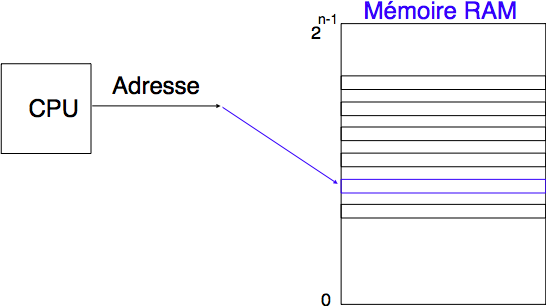
\includegraphics[width=\linewidth]{proc-mem.png}
    \caption{Modèle simple d'interaction entre le processeur et la
    mémoire}
\end{figure}

Ce modèle correspond au fonctionnement de processeurs simples tels que
ceux que l'on trouve sur des systèmes embarqués comme une machine à
lessiver. Malheureusement, il ne permet pas d'expliquer et de
comprendre le fonctionnement des ordinateurs actuels. Pour s'en
convaincre, il suffit de réfléchir à quelques problèmes liés à
l'utilisation de la mémoire sur un ordinateur fonctionnant sous Unix.
\newline
 
Le premier problème est lié à l'organisation d'un processus en mémoire.
Sous Unix, le bas de la mémoire est réservé au code, le milieu au heap
et le haut au stack. Le modèle simple d'organisation de la mémoire ne
permet pas facilement de comprendre comment un tel processus peut
pouvoir utiliser la mémoire sur un processeur 64 bits qui est placé
dans un ordinateur qui ne dispose que de 4 GBytes de mémoire. Avec une
telle quantité de mémoire, le sommet de la pile devrait se trouver à
une adresse proche de $2^{32}$ et non $2^{64}$.
\newline
 
Un deuxième problème est lié à l'utilisation de plusieurs processus
simultanément en mémoire. Lorsque deux processus s'exécutent, ils
utilisent nécessairement la même mémoire physique. Si un processus
utilise l'adresse $x$ et y place des instructions ou des données,
cette adresse ne peut pas être utilisée par un autre processus.
Physiquement, ces deux processus doivent utiliser des zones mémoires
distinctes. Pourtant, le programme ci-dessous affiche les adresses de
\verb#argc#, de la fonction \verb#main# et de la fonction \verb#printf# de la
librairie standard puis effectue \verb#sleep(20);#. Lors de l'exécution de
deux instances de ce programmes simultanément, on observe ceci sur la
sortie standard. \newline

\begin{lstlisting}[language=bash]
$ ./simple &
 [pid=32955] Adresse de argc : 0x7fff5fbfe18c
 [pid=32955] Adresse de main : 0x100000e28
 [pid=32955] Adresse de printf : 0x7fff8a524f3a
$ ./simple 2 3 4
 [pid=32956] Adresse de argc : 0x7fff5fbfe18c
 [pid=32956] Adresse de main : 0x100000e28
 [pid=32956] Adresse de printf : 0x7fff8a524f3a
\end{lstlisting}
 
Manifestement, les deux programmes utilisent exactement les mêmes
adresses en mémoire. Pourtant, ces deux programmes doivent
nécessairement utiliser des zones mémoires différentes pour pouvoir
s'exécuter correctement. Ceci est possible grâce à l'utilisation de la
\textit{émoire virtuelle}. Avec la \textit{mémoire virtuelle}, deux
types d'adresses sont utilisées sur le système : les \textbf{adresses
virtuelles} et les \textbf{adresses réelles} ou \textbf{physiques}. Une
\textit{adresse virtuelle} est une adresse qui est utilisée à
l'intérieur d'un programme. Les adresses des variables ou des fonctions
de notre programme d'exemple ci-dessus sont des adresses virtuelles.
Une \textit{adresse physique} est l'adresse qui est utilisée par des
puces de RAM pour les opérations d'écriture et de lecture. Ce sont les
adresses physiques qui sont échangées sur le bus auquel la mémoire est
connectée. Pour que les programmes puissent accéder aux instructions et
données qui se trouvent en mémoire, il est nécessaire de pouvoir
traduire les adresses virtuelles en adresses physiques. C'est le rôle
du \textbf{MMU} ou \textbf{Memory Management Unit}.
Historiquement, le \textit{MMU} était implémenté sous la forme
d'un chip séparé qui était placé entre le processeur (qui utilisait
alors des adresses virtuelles) et la mémoire (qui utilise elle toujours
des adresses physiques). Aujourd'hui, le \textit{MMU} est
directement intégré au processeur pour des raisons de performance, mais
conceptuellement son rôle reste essentiel comme nous allons le voir.
\newline
 
Le rôle principal du \textit{MMU} est de traduire toute adresse
virtuelle en une adresse physique. Avant d'expliquer comment le
\textit{MMU} peut être implémenté en pratique, il est utile de
passer en revue plusieurs avantages de l'utilisation des adresses
virtuelles.
 
\begin{figure}[!ht] 
    \centering
    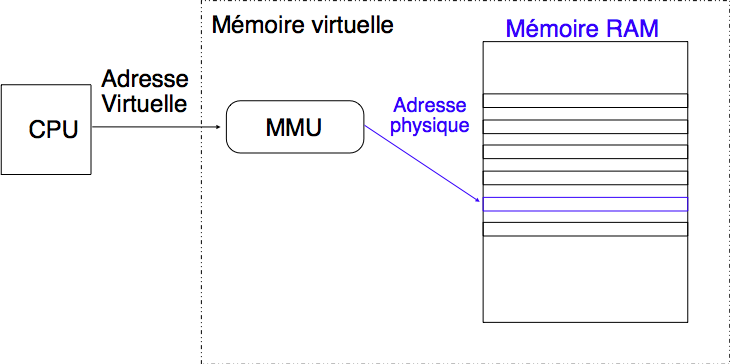
\includegraphics[width=\linewidth]{mmu.png}
    \caption{MMU et mémoire virtuelle}
\end{figure}
   
Un premier avantage de l'utilisation de la mémoire virtuelle est
qu'elle permet de découpler les adresses virtuelles des adresses
physiques. Celles-ci ne doivent pas nécessairement être encodées en
utilisant le même nombre de bits. La longueur des adresses dépend
généralement de l'architecture du processeur et de la taille des
registres qu'il utilise. Une organisation possible de la mémoire
virtuelle est d'utiliser des adresses virtuelles qui sont encodées
sur autant de bits que les adresses physiques, mais ce n'est pas la
seule. Il est tout à fait possible d'avoir un ordinateur sur lequel
les adresses virtuelles sont plus longues que les adresses physiques.
C'est le cas par exemple sur les ordinateurs bon marché qui utilisent
une quantité réduite de mémoire RAM. Inversement, la mémoire
virtuelle permet à un serveur d'utiliser des adresses physiques qui
sont plus longues que les adresses virtuelles. Cela lui permet
d'utiliser une capacité de mémoire plus importante que celle
autorisée par l'architecture de son processeur. Dans ce cas, un
processus ne peut pas utiliser plus de mémoire que l'espace
d'adressage virtuel disponible. Mais ensemble, tous les processus
fonctionnant sur l'ordinateur peuvent utiliser tout l'espace
d'adressage physique disponible. \newline

Un deuxième avantage de la mémoire virtuelle est qu'elle permet, à
condition de pouvoir réaliser une traduction spécifique à chaque
processus, de partager efficacement la mémoire entre plusieurs
processus tout en leur permettant d'utiliser les mêmes adresses
virtuelles. C'est cette particularité de la mémoire virtuelle qui
nous a permis dans l'exemple précédent d'avoir deux processus qui en
apparence utilisent les mêmes adresses. En effectuant une traduction
spécifique à chaque processus, le \textit{MMU} permet d'autres
avantages qui sont encore plus intéressants.\newline
   
Le \textit{MMU} est capable d'effectuer des traductions d'adresses
virtuelles qui sont spécifiques à chaque processus. Cela implique
qu'en général la traduction de l'adresse $x$ dans le processus $P1$
ne donnera pas la même adresse physique que la traduction de
l'adresse $x$ dans le processus $P2$. Par contre, il est tout à fait
possible que la traduction de l'adresse $w$ (resp. $y$) dans le processus
$P1$ (resp. $P2$) donne l'adresse physique $z$ dans les deux processus.
Comme nous le verrons ultérieurement,
cela permet à deux processus distincts de partager de la mémoire.
Cette propriété est aussi à la base du fonctionnement des librairies
partagées dans un système Unix. Dans notre exemple, la fonction
\verb#printf# qui est utilisée par les deux processus fait partie de la
librairie standard. Celle-ci doit être chargée en mémoire lors de
l'exécution de chacun des processus. Grâce à l'utilisation du
\textit{MMU} et de la mémoire virtuelle, une seule copie physique
de la librairie standard est chargée en mémoire et tous les processus
qui y font appel utilisent les instructions se trouvant dans cette
copie physique. Cela permet de réduire fortement la consommation de
mémoire lorsque de nombreux processus s'exécutent simultanément, ce
qui est souvent le cas sur un système Unix. \newline
   
Le dernier avantage de l'utilisation de la mémoire virtuelle est
qu'il est possible de combiner ensemble la mémoire RAM et un ou des
dispositifs de stockage tels que des disques durs ou des disques SSD
pour constituer une mémoire virtuelle de plus grande capacité que la
mémoire RAM disponible. Pour cela, il suffit, conceptuellement, que
le \textit{MMU} soit capable de supporter deux types d'adresses
physiques : les adresses physiques en RAM et les adresses physiques
qui correspondent à des données stockées sur un dispositif de
stockage \footnote{En pratique, les adresses sur le disque dur ne sont
pas stockées dans le \textit{MMU} mais dans une table maintenue par
le système d'exploitation. C'est le noyau qui est responsable des
transferts entre le dispositif de stockage et la mémoire RAM}. \newline

\begin{figure}
    \centering
    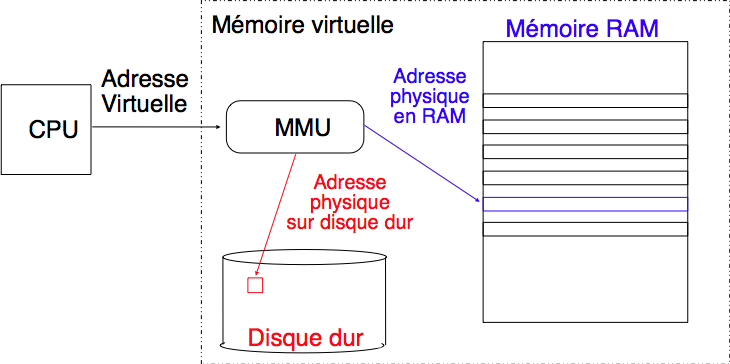
\includegraphics[width=\linewidth]{vmem.png}
    \caption{Organisation de la \textit{mémoire virtuelle}}
\end{figure}

Cette possibilité de combiner la mémoire RAM et les dispositifs de
stockage offre encore plus de possibilités. Comme nous le verrons, grâce
à la mémoire virtuelle, un processus pourra accéder à des fichiers via
des pointeurs et des écriture/lectures en mémoire. Le chargement d'un
programme pourra s'effectuer en passant par la mémoire virtuelle de
façon à charger uniquement les parties du programme qui sont nécessaires
en mémoire. Nous verrons également qu'il existe plusieurs appels
systèmes qui permettent à des processus de contrôler leur utilisation de
la mémoire virtuelle. \newline

\subsubsection{Fonctionnement de la mémoire virtuelle}

Avant d'analyser comment la mémoire virtuelle peut être utilisée par les
processus, il est important de bien comprendre son organisation et les
principes de base de fonctionnement du \textit{MMU}. La mémoire
virtuelle combine la mémoire RAM et les dispositifs de stockage. Comme
la mémoire RAM et les dispositifs de stockage ont des caractéristiques
fort différentes, il n'est pas trivial de les combiner pour donner
l'illusion d'une mémoire virtuelle unique.\newline

Au niveau de l'adressage, la mémoire RAM permet d'adresser des octets et
supporte des lectures et des écritures à n'importe quelle adresse. La
mémoire RAM permet au processeur d'écrire et de lire des octets ou des
mots à une position déterminée en mémoire.\newline

Un dispositif de stockage (disque dur, CD/DVD, \ldots) quant à lui
contient un ensemble de secteurs. Chaque secteur peut être identifié par
une adresse, comprenant par exemple le numéro du plateau, le numéro de
la piste et le numéro du secteur sur la piste. Sur un tel dispositif, le
secteur est l'unité de transfert de l'information. Cela implique que la
moindre lecture/écriture sur un dispositif de stockage nécessite la
lecture/écriture d'au moins 512 octets, même pour modifier un seul bit.
Enfin, la dernière différence importante entre ces deux technologies est
leur temps d'accès. Au niveau des mémoires RAM, les temps d'accès sont
de l'ordre de quelques dizaines de nanosecondes. Pour un dispositif de
stockage, les temps d'accès peuvent être de quelques dizaines de
microsecondes pour un dispositif de type \textit{Solid State Drive}
ou \textit{SSD} et jusqu'à quelques dizaines de millisecondes pour un
disque dur. Les tableaux ci-dessous présentent les caractéristiques
techniques de deux dispositifs de stockage \footnote{Source :
    \url{http://www.intel.com/content/www/us/en/solid-state-drives/ssd-320-specification.html}}
    \footnote{Source :
        \url{http://www.seagate.com/staticfiles/support/disc/manuals/desktop/Barracuda\%207200.11/100507013e.pdf}} à titre d'exemple.\newline

La mémoire virtuelle utilise elle une unité intermédiaire qui est la
\textit{page}. Une \textbf{page} est une zone de mémoire contigüe. La
taille des pages dépend de l'architecture du processeur et/ou du système
d'exploitation utilisé. Une taille courante est de 4096 octets. \newline

\begin{lstlisting}[language=C]
#include <unistd.h>
   int sz = getpagesize();
\end{lstlisting} 

Lorsqu'un programme est chargé en mémoire, par exemple lors de
l'exécution de l'appel système \verb#execve(2)#, il est
automatiquement découpé en pages. Grâce à la mémoire virtuelle, ces
pages peuvent être stockée dans n'importe quelle zone de la mémoire
RAM. La seule contrainte est que tous les octets qui font partie de la
même page soient stockés à des adresses qui sont contigües. Cette
contrainte permet de structurer les adresses virtuelles en deux
parties comme représenté dans la figure ci-dessous. Une
\textit{adresse virtuelle} est donc un ensemble de bits. Les bits
de poids fort servent à identifier la \textit{page} dans laquelle une
donnée est stockée. Les bits de poids faible (12 lorsque l'on utilise
des pages de 4 KBytes), identifient la position de la donnée par
rapport au début de la page. \newline
  
\begin{figure}[!ht]
    \centering
    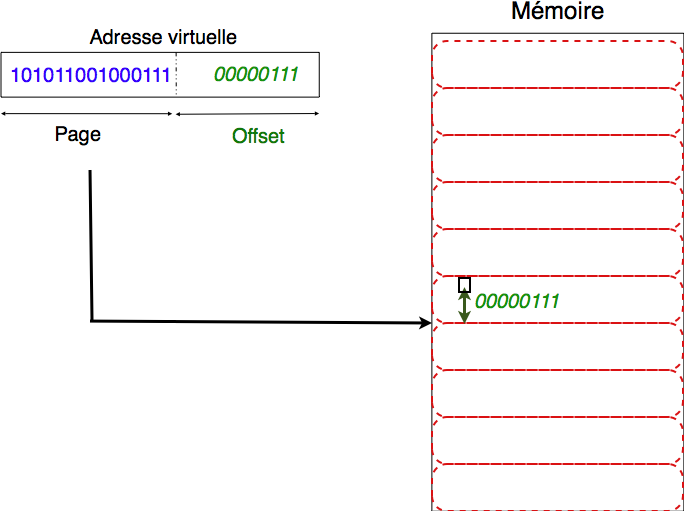
\includegraphics[width=\linewidth]{addrvirtuelle.png}
    \caption{Adresse virtuelle}
\end{figure}
   
Grâce à cette organisation des adresses virtuelles, il est possible
de construire un mécanisme efficace qui permet de traduire une
adresse virtuelle en une adresse réelle. La première solution qui a
été proposée pour réaliser cette traduction est d'utiliser une
\textbf{table des pages}. La \textbf{table des pages} est stockée
en mémoire RAM et contient une ligne pour chaque page appartenant à
la mémoire virtuelle. A titre d'exemple, un système utilisant des
adresses virtuelles de 32 bits et des pages de 4 KBytes contient
$2^{32-12} =2^{20}$ pages. La table des pages de ce système
contient donc $2^{20}$ lignes. Une ligne de la table des
pages contient différentes informations que nous détaillerons par
après. Les deux plus importantes sont :
   
\begin{itemize}
    \item le \textbf{bit de validité} qui indique si la page est
        actuellement présente en mémoire RAM ou non
    \item l'adresse en mémoire RAM à laquelle la page est actuellement
        stockée (si elle est présente en mémoire RAM, sinon une
        information permettant de trouver la page sur un dispositif de
        stockage)
\end{itemize}
 
La table des page est stockée en mémoire RAM comme un tableau en C.
L'information correspondant à la page $0$ est stockée à l'adresse
de début de la table des pages. Cette adresse de début de la table des
pages ($P$) est généralement stockée dans un registre du processeur
pour être facilement accessible. Si une entrée \footnote{Une entrée de
la table de pages occupe généralement 32 ou 64 bits suivant les
architectures de processeurs} de la table
des pages est encodée en $n$ bytes, l'information correspondant à la
page $1$ sera stockée à l'adresse $P + n$, celle relative à la page
$2$ à l'adresse $P+2*n$, \ldots Cette organisation permet
d'accéder facilement à l'entrée de la table des pages relative à la
page $z$. Il suffit en effet d'y accéder depuis l'adresse $P+z*n$.
 
Grâce à cette table des pages, il est possible de traduire directement
les adresses virtuelles en adresses physiques. Cette traduction est
représentée dans la figure ci-dessous. Pour réaliser une traduction, il
faut tout d'abord extraire de l'adresse virtuelle le numéro de la page.
Celui-ci se trouve dans les bits de poids fort de l'adresse virtuelle.
Le numéro de la page sert d'index pour récupérer l'entrée correspondant
à cette page dans la table des pages. Cette entrée contient l'adresse
en mémoire RAM à laquelle la page débute. Pour finaliser la traduction
de l'adresse virtuelle, il suffit de concaténer les bits de poids
faible de l'adresse virtuelle avec l'adresse de la page en mémoire RAM.
Cette concaténation donne l'adresse réelle à laquelle la donnée est
stockée en mémoire RAM. Cette adresse physique permet au processeur
d'accéder directement à la donnée en mémoire. \newline
 
\begin{figure}[!ht]
    \centering
    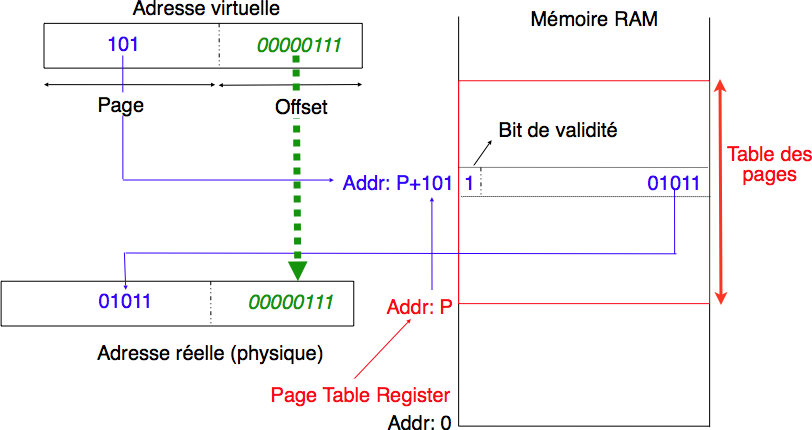
\includegraphics[width=\linewidth]{traduction.png}
    \caption{Traduction d'adresses avec une table des pages}
\end{figure}
  
La table des pages permet de traduire les adresses virtuelles en
adresses physiques. Ce faisant, elle introduit un mécanisme
d'indirection entre les adresses (virtuelles) qui sont utilisées par
les programmes et les adresses (réelles) qui sont utilisées par le
hardware. Ce mécanisme d'indirection a de nombreuses applications
comme nous le verrons par la suite.\newline
  
Un point important à mentionner concernant l'utilisation d'un
mécanisme de traduction des adresses est qu'il permet de  découpler le
choix de la taille des adresses (virtuelles) utilisées par les
programmes des contraintes matérielles qui sont liées directement aux
mémoires RAM utilisées. En pratique, il est très possible d'avoir des
systèmes informatiques dans lesquels les adresses virtuelles sont plus
longues, plus courtes ou ont la même longueur que les adresses
physiques. Sur un ordinateur 32 bits actuel équipé de 4 GBytes de
mémoire, il est naturel d'utiliser des adresses virtuelles de 32 bits
et des adresses physiques de 32 bits également pour pouvoir accéder à
l'ensemble de la mémoire. Dans ce cas, la mémoire virtuelle permet
d'accéder à toute la mémoire physique. Aujourd'hui, il existe des
serveurs 64 bits. Ceux-ci utilisent des adresses virtuelles de 64
bits, mais aucun ordinateur ne contient $2^{64}$ bytes de
mémoire. Par exemple, un serveur disposant de 128 GBytes de mémoire
physique pourrait se contenter d'utiliser des adresses physiques de 37
bits. Dans ce cas, la mémoire virtuelle donne l'illusion qu'il est
possible d'accéder à plus de mémoire que celle qui est réellement
disponible. D'un autre côté, il est aussi possible de construire des
serveurs qui utilisent des adresses virtuelles de 32 bits, mais
disposent de plus de 4 GBytes de mémoire RAM. Dans ce cas, les
adresses physiques pourront être plus longues que les adresses
réelles. Quelles que soient les longueurs respectives des adresses
virtuelles et physiques, la table des pages, sous le contrôle du
système d'exploitation, permettra de réaliser efficacement les
traductions entre les adresses virtuelles et les adresses physiques.
\newline
  
Pour bien comprendre la traduction des adresses virtuelles en
utilisant la table des pages, considérons un système imaginaire qui
utilise des adresses virtuelles encodées sur 7 bits et des adresses
physiques qui sont elles encodées sur 6 bits. La table des pages
correspondante est reprise dans le tableau ci-dessous. Comme dans la
figure précédente, la ligne du bas du tableau est relative à la page
$0$.

\bigskip
\begin{tabular}{|l|l|}
    \hline
    Validité & Adresse \\
    \hline
    true & 00 \\
    false & - \\
    true & 11 \\
    false & - \\
    false & - \\
    false & - \\
    true & 01 \\
    true & 10 \\
    \hline
\end{tabular}
\bigskip

Cette mémoire virtuelle contient quatre pages. La première couvre les
adresses physiques allant de \verb#000000# à \verb#001111#, la seconde de
\verb#010000# à \verb#011111#, la troisième de \verb#100000# à
\verb#101111# et la dernière de \verb#110000# à \verb#111111#. Les
adresses virtuelles elles vont de \verb#0000000# à \verb#1111111#. La
traduction s'effectue sur base
de la table des pages. Ainsi, l'adresse \verb#1010001# correspond à
l'octet \verb#0001# dans la page virtuelle \verb#101#. Sur base la table
des pages, cette page se trouve en mémoire RAM (sont bit de validité
est vrai) et elle démarre à l'adresse \verb#110000#. L'adresse virtuelle
\verb#1010001# est donc traduite en l'adresse réelle \verb#110001#.
L'adresse virtuelle \verb#0110111# correspond elle à une page qui n'est
pas actuellement en mémoire RAM puisque le bit de validité
correspondant à la page \verb#011# est faux.\newline
   
Si on analyse la table des pages ci-dessus, on peut remarquer que la
page contenant les adresses virtuelles les plus hautes se trouve dans
la zone mémoire avec les adresses physiques les plus basses.
Inversement, la page qui est en mémoire RAM à l'adresse la plus
élevée correspond à des adresses virtuelles qui se trouvent au milieu
de l'espace d'adressage. Ce découplage entre l'adresse virtuelle et
la localisation physique de la page en mémoire est un des avantages
importants de la mémoire virtuelle.\newline
   
La mémoire virtuelle a aussi un rôle important à jouer lorsque
plusieurs processus s'exécutent simultanément.
Comme indiqué ci-dessus, l'adresse de la table des pages est stockée
dans un des registre du processeur. L'utilisation de ce registre
permet d'avoir une table des pages pour chaque processus. Pour cela,
il suffit qu'une zone de mémoire RAM soit réservée pour chaque
processus et que le système d'exploitation y stocke la table des
pages du processus. Lors d'un changement de contexte, le système
d'exploitation modifie le registre de table des pages de façon à ce
qu'il pointe vers la table des pages du processus qui s'exécute. Ce
mécanisme est particulièrement utile et efficace.\newline
   
A titre d'exemple, considérons un système imaginaire utilisant des
adresses virtuelles sur 6 bits et des adresses physiques sur 8 bits.
Deux processus s'exécutent sur ce système et ils utilisent chacun
trois pages, deux pages dans le bas de l'espace d'adressage virtuel
qui correspondent à leur segment de code et une page dans le haut de
l'espace d'adressage virtuel qui correspond à leur pile. Le premier
tableau ci-dessous présente la table des pages du processus
$P1$.\newline

\bigskip
\begin{tabular}{|l|l|}
    \hline
    Validité & Adresse \\
    \hline
    true & 0011 \\
    false & - \\
    true & 1001 \\
    true & 1000 \\
    \hline
\end{tabular}
\bigskip

Le processus $P2$ a lui aussi sa table des pages. Celle-ci pointe
vers des adresses physiques qui sont différentes de celle utilisées
par le processus $P1$. L'utilisation d'une table des pages par
processus permet à deux processus distincts d'utiliser les mêmes
adresses virtuelles.\newline

\bigskip
\begin{tabular}{|l|l|}
    \hline
    Validité & Adresse \\
    \hline
    true & 0000 \\
    false & - \\
    true & 1111 \\
    true & 1110 \\
    \hline
\end{tabular}
\bigskip

Lorsque le processus $P1$ s'exécute, c'est sa table des pages qui
est utilisée par le processeur pour la traduction des adresses
virtuelles en adresses physiques. Ainsi, l'adresse \verb#011101# est
traduite en l'adresse \verb#10011101#. Par contre, lorsque le processus
$P2$ s'exécuté, cette adresse \verb#011101# est traduite grâce à  la
table des pages de ce processus en l'adresse \verb#11111101#.

\begin{framed}
    \textbf{Note} : Performance de la mémoire virtuelle \newline

    Grâce à son mécanisme d'indirection entre les adresses virtuelles
    et les adresses physiques, la mémoire virtuelle permet de nombreuses
    applications comme nous le verrons dans les sections qui suivent.
    Cependant, la mémoire virtuelle peut avoir un impact important au
    niveau des performances des accès à une donnée en mémoire. Pour cela,
    il est intéressant d'analyser en détails ce qu'il se passe lors de
    chaque accès à la mémoire. Pour accéder à une donnée en mémoire, le
    \textbf{MMU} doit d'abord consulter la table des pages pour
    traduire l'adresse virtuelle en une adresse physique correspondante.
    Ce n'est qu'après avoir obtenu cette adresse physique que le
    processeur peut effectuer l'accès à la mémoire RAM. En pratique,
    l'utilisation d'une table des pages a comme conséquence de doubler le
    temps d'accès à une donnée en mémoire. Lorsque la mémoire virtuelle a
    été inventée, ce doublement du temps d'accès à la mémoire n'était pas
    une limitation car les mémoires RAM étaient nettement plus rapides que
    les processeurs. Aujourd'hui, la situation est complètement inversée
    puisque les processeurs sont déjà fortement ralentis par les temps
    d'accès à la mémoire RAM. Doubler ce temps d'accès aurait un impact
    négatif sur les performances des processeurs. Pour faire face à ce
    problème, les processeurs actuels disposent tous d'un
    \textit{Translation Lookaside Buffer} (\textbf{TLB}). Ce
    \textit{TLB} est en fait une sorte de \textit{mémoire cache} qui permet
    de stocker dans une mémoire rapide se trouvant sur le processeur
    certaines lignes de la \textbf{table des pages}. Les détails de
    gestion du \textit{TLB} sortent du cadre de ce cours. Grâce à
    l'utilisation du \textit{TLB} la plupart des traductions des
    adresses virtuelles en adresses physique peuvent être obtenus sans
    devoir directement consulter la table des pages.
\end{framed}
  
La table des pages d'un processus contrôle les adresses physiques
auxquelles le processus a accès. Pour garantir la sécurité d'un
système informatique, il faut bien entendu éviter qu'un processus ne
puisse modifier lui-même et sans contrôle sa table des pages. Toutes
les manipulations de la table des pages ou du registre de table des
pages se font sous le contrôle du système d'exploitation. La
modification du registre de table des pages est une opération
privilégiée qui ne peut être exécutée que par le système
d'exploitation. \newline
  
En termes de sécurité, une entrée de la table des pages contient
également des bits de permission qui sont contrôlés par le système
d'exploitation et spécifient quelles opérations peuvent être
effectuées sur chaque page. Une entrée de la table des pages contient
trois bits de permissions : \newline

\begin{itemize}
    \item $R$ bit. Ce bit indique si le processus peut accéder en
        lecture à la page se trouvant en mémoire physique.
    \item $W$ bit. Ce bit indique si le processus peut modifier le
        contenu de la page se trouvant en mémoire physique
    \item $X$ bit. Ce bit indique si la page contient des instructions qui
        peuvent être exécutées par le processeur ou des données.
\end{itemize}
 
Ces bits de protection sont généralement fixés par le système
d'exploitation. Par exemple, le segment code qui ne contient que des
instructions à exécuter pourra être stocké dans des pages avec les bits
$R$ et $X$ mais pas le bit $W$ pour éviter que le processus ne
modifie les instructions qu'il exécute. Le stack par contre sera placé
dans des pages avec les bits $R$ et $W$ mais pas le bit $X$. Cette
technique est utilisée dans les systèmes d'exploitation récents pour
éviter qu'un problème de buffer overflow sur le stack ne conduise à
l'exécution d'instructions qui ne font pas partie du processus. Le heap
peut utiliser les mêmes bits de protection. Enfin, les pages qui n'ont
pas été allouées au processus, notamment celles se trouvant entre le
heap et le stack auront toutes leurs bits de protection mis à faux.
Cela permet au processeur de détecter les accès à de la mémoire qui n'a
as été allouée au processus. Un tel accès provoquera la génération
d'une \textit{segmentation fault} et l'envoi du signal
correspondant.\newline
 
Même si ces bits de protection sont contrôlés par le système
d'exploitation, il est parfois utile à un processus de modifier les
bits de permissions qui sont associés à certaines de ses pages. Cela
peut se faire via l'appel système \verb#mprotect(2)#.\newline

\begin{lstlisting}[language=C]
#include <sys/mman.h>
int mprotect(const void *addr, size_t len, int prot);
\end{lstlisting}
   
Cet appel système prend trois arguments. Le première est un pointeur
vers le début de la zone mémoire dont il faut modifier les bits de
protection. Le second est la longueur de la zone mémoire concernée et
le dernier la protection souhaitée. Celle-ci est spécifiée en
utilisant les constantes \verb#PROT_NONE#, \verb#PROT_READ#,
\verb#PROT_WRITE# et \verb#PROT_EXEC# qui peuvent être combinées en utilisant une
disjonction logique. La protection demandée ne peut pas être plus
libérale que la protection qui est déjà fixée par le système
d'exploitation. Dans ce cas, le système d'exploitation génère un
signal \verb#SIGSEGV#.\newline
   
\subsubsection{Utilisation des dispositifs de stockage}
 
La mémoire virtuelle permet non seulement à des pages d'un processus
d'être placées à différents endroits de la mémoire, mais aussi elle
permet de combiner la mémoire RAM et les dispositifs de stockage de
façon transparente pour les processus.\newline
   
Une partie des pages qui composent la mémoire virtuelle peut être
stockée sur un dispositif de stockage (disque dur, SSD, \ldots). En
pratique, la mémoire RAM peut jouer le rôle d'une sorte de mémoire
cache pour la mémoire virtuelle. Les pages qui sont le plus
fréquemment utilisées sont placées en mémoire RAM par le système
d'exploitation et les pages les moins utilisées sont elles placées
sur un dispositif de stockage et ramenées en mémoire RAM lorsqu'elle
sont utilisées par le processeur.\newline
   
Pour bien comprendre cette utilisation de la mémoire virtuelle, il
nous faut revenir à la table des pages. Celle-ci comprend autant
d'entrées qu'il y a de pages dans l'espace d'adressage d'un
processus. Nous avons vu qu'une entrée de cette table pouvait être
structurée comme dans la figure ci-dessous.\newline

\begin{figure}[!ht]
    \centering
    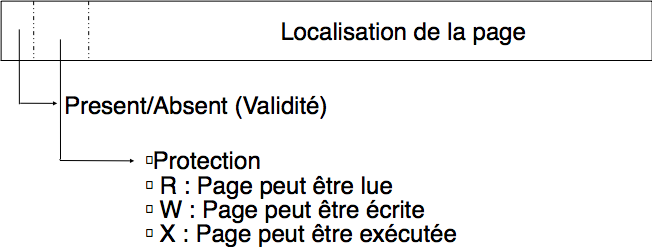
\includegraphics[width=\linewidth]{entreeTable.png}
    \caption{Entrée de la table des pages}
\end{figure}

Le bit de validité indique si la page est présente en mémoire RAM ou
non. Lorsque la page est présente en mémoire RAM, les bits de poids
faible de l'entrée de la table des pages contiennent l'adresse physique
de la page en mémoire RAM. Lorsque le bit de validité a comme valeur
\textit{faux} cela signifie que la page n'existe pas (elle n'a
jamais été créée) ou qu'elle est actuellement stockée sur un dispositif
de stockage. Si la page n'existe pas, aucun de ses bits de permission
n'aura comme valeur \textit{vrai} et tout accès à cette page provoquera
une \textit{segmentation fault}. Si par contre la page existe mais se
trouve sur un dispositif de stockage, alors l'information de
localisation pointera vers une structure de données qui est maintenue
par le système d'exploitation et contient la localisation physique de la
donnée sur un dispositif de stockage.\newline

Schématiquement, ces informations de localisation des pages peuvent être
de deux types. Lorsqu'un dispositif de stockage, ou une partition d'un
tel dispositif, est dédié au stockage de pages de la mémoire virtuelle,
alors la localisation d'une page est composée de l'identifiant du
dispositif et du numéro du secteur sur le dispositif. Ce sera le cas
lorsque par exemple une \textbf{partition de swap} est utilisée. Sous
Linux, le fichier ``/proc/swaps`` contient la liste des partitions de
swap qui sont utilisées pour stocker les pages de la mémoire virtuelle
avec leur type, leur taille et leur utilisation. Une telle partition de
swap peut être créée avec l'utilitaire \verb#mkswap(8)#. Elle est
activée en exécutant la commande \verb#swapon(8)#. Celle-ci est
généralement lancée automatiquement lors du démarrage du
système.\newline

\begin{lstlisting}[language=bash]
$ cat /proc/swaps
Filename Type Size Used Priority
/dev/sda3            partition 8193140 444948 -1
\end{lstlisting}
 
Outre les partitions de swap, il est également possible de stocker des
pages de la mémoire virtuelle dans des fichiers. Dans ce cas, la
localisation d'une page comprend le dispositif, l'\textbf{inode} du
fichier et l'offset à partir duquel la page est accessible dans le
fichier. En pratique, les partitions de swap sont un peu plus rapides
que les fichiers de swap car les secteurs qui composent une telle
partition sont contigus, ce qui n'est pas toujours le cas avec un
fichier de swap. D'un autre côté, il est plus facile d'ajouter ou de
retirer des fichiers de swap que des partitions de swap sur un
dispositif de stockage. En pratique, les deux techniques peuvent être
utilisées.\newline
 
A ce stade, il est utile d'analyser à nouveau le fonctionnement de la
mémoire virtuelle. En toute généralité, celle-ci est découpée en pages
et comprend une mémoire RAM et un ou plusieurs dispositifs de stockage.
Pour simplifier la présentation, nous supposons qu'un seul disque dur
est utilisé.\newline

\begin{figure}[!ht]
    \centering
    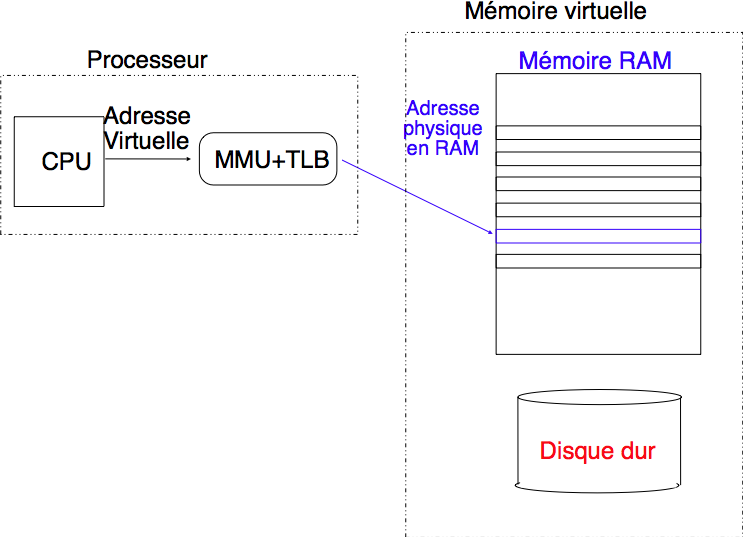
\includegraphics[width=\linewidth]{memoireVirtuelle.png}
    \caption{La mémoire virtuelle}
\end{figure}

Les processus utilisent des adresses virtuelles pour représenter les
positions des données et des instructions en mémoire virtuelles. Ces
adresses virtuelles sont donc utilisées par le CPU chaque fois qu'il
doit charger ou sauvegarder une donnée ou une instruction en mémoire.
Comme nous l'avons vu, le \textit{MMU} permet de traduire les
adresses virtuelles en adresses réelles. Pour des raisons de
performance, le \textit{MMU} est intégré directement sur le
processeur et il comprend un \textit{TLB} qui sert de cache pour les
entrées de la table des pages du processus qui est en train de
s'exécuter.\newline
  
Considérons une opération de lecture faite par le CPU. Pour réaliser
cette opération, le CPU fournit l'adresse virtuelle au
\textit{MMU}. Celui-ci va consulter le \textit{TLB} pour traduire
l'adresse virtuelle demandée. Cette traduction peut nécessiter
différentes opérations. Supposons que l'entrée de la table des pages
demandées se trouve dans le \textit{TLB}.
  
\begin{itemize}
    \item Si le \textit{bit de validité} de la page est \textit{vrai},
        la page demandée se situe en mémoire RAM. Dans ce cas, le
        \textit{MMU} vérifie via les bits de permissions si l'accès
        demandé (dans ce cas une lecture, mais un raisonnement similaire
        est valable pour une écriture ou le chargement d'une
        instruction) est valide.
    \item Si l'accès est autorisé, le \textit{MMU} retourne l'adresse
        réelle et le processeur accède aux données.
    \item Si l'accès n'est pas autorisé, le processeur génère une
        interruption. Le processus ayant tenté d'accéder à une zone de
        mémoire ne faisant pas partie de son espace d'adressage virtuel,
        c'est au système d'exploitation de réagir. Celui-ci enverra un
        signal segmentation fault, \verb#SIGSEGV#, au processus qui a tenté cet accès.
    \item Si le \textit{bit de validité} de la page est faux, la page
        demandée ne se trouve pas en mémoire RAM.

        Deux cas de figure sont possibles :
        \begin{itemize}
            \item les bits de permission ne permettent aucun accès à la
                page. Dans ce cas, la page n'existe pas et le
                \textit{MMU} va générer une interruption qui va
                provoquer l'exécution d'une routine de   traitement
                d'interruption du système d'exploitation. Lors du
                traitement de cette opération, le noyau va envoyer un
                signal   segmentation fault au processus qui a tenté cet
                accès.
            \item les bits de permission permettent l'accès à la page.
                On parle dans ce cas de \textit{page fault} c'est-à-dire
                qu'une page nécessaire à l'exécution du processus n'est
                pas disponible en mémoire RAM. Vu les temps d'accès et
                la complexité d'accéder à une page sur un disque dur
                (via une partition, un fichier de swap ou un fichier
                normal), le \textit{MMU} ne peut pas accéder directement
                à la donnée sur le disque dur. Le \textit{MMU} va donc
                générer une interruption qui va forcer l'exécution d'une
                routine de traitement d'interruption par le noyau. Cette
                routine va identifier la page manquante et préparer son
                transfert du disque dur vers la mémoire. Ce transfert
                peut durer plusieurs dizaines de millisecondes, ce qui
                est un temps très long par rapport à l'exécution
                d'instructions par le processeur. Tant que cette page
                n'est pas disponible en mémoire RAM, le processus ne
                peut continuer son exécution. Il passe dans l'état
                bloqué et le noyau effectue un changement de contexte
                pour exécuter un autre processus. Lorsque la page
                manquante aura été rapatriée depuis le disque dur en
                mémoire RAM, le noyau pourra relancer le processus qu'il
                avait bloqué afin de retenter l'accès mémoire qui vient
                d'échouer.
        \end{itemize}
\end{itemize}
   
Durant son exécution, un système doit pouvoir gérer des pages qui se
trouvent en mémoire RAM et des pages qui sont stockées sur le disque
dur. Lorsque la mémoire RAM en entièrement remplies de pages, il peut
être nécessaire d'y libérer de l'espace mémoire et déplaçant des
pages vers un des dispositifs de stockage. C'est le rôle des
algorithmes de remplacement de pages.
   
\subsubsection{Stratégies de remplacements de pages}

C'est le système d'exploitation qui prend en charge les transferts de
pages entre les dispositifs de stockage et la mémoire. Tant que la
mémoire RAM n'est pas remplie, ces transferts sont simples, il suffit
de ramener une ou plusieurs pages du dispositif de stockage vers la
mémoire RAM. En général, le système d'exploitation cherchera à
exploiter le principe de localité lors de ces transferts. Lorsqu'une
page manque en mémoire RAM, le noyau programmera le chargement de
cette page, mais aussi d'autres pages du même processus ayant des
adresses proches.\newline
   
Lorsque la mémoire RAM est remplie et qu'il faut ramener une page
depuis un dispositif de stockage, le problème est plus délicat. Pour
pouvoir charger cette nouvelle page en mémoire RAM, le système
d'exploitation doit libérer de la mémoire. Pour cela, il doit
implémenter une \textit{stratégie de remplacement des pages} en
mémoire. Cette stratégie définit quelle page doit être
préférentiellement retirée de la mémoire RAM et placée sur le
dispositif de stockage. Différentes stratégies sont possibles. Elles
résultent en général d'un compromis entre la quantité d'information
de contrôle qui est stockée dans la table des pages et les
performances de la stratégie de remplacement des pages. \newline
   
Une première stratégie de remplacement de pages pourrait être de
sauvegarder les identifiants des pages dans une \textit{file FIFO}.
Chaque fois qu'une page est créée par le noyau, son identifiant est
placé à la fin de la \textit{file FIFO}. Lorsque la mémoire est pleine
et qu'une page doit être retirée de la mémoire RAM, le noyau pourrait
choisir la page dont l'identifiant se trouve en tête de la \textit{file
FIFO}. Cette stratégie a l'avantage d'être simple à implémenter, mais
remettre sur disque la page la plus anciennement créée n'est pas
toujours la solution la plus efficace du point de vue des performances.
En effet, cette page peut très bien être une des pages les plus
utilisées par le processeur. Si elle est remise sur le disque, elle
risque de devoir être récupérée peu de temps après.\newline
   
Au niveau des performances, la meilleure stratégie de remplacement de
pages serait de sauvegarder sur le disque dur les pages qui seront
utilisées par le processeur d'ici le plus de temps possible.
Malheureusement, cette stratégie nécessite de prévoir le futur, une
fonctionnalité qui n'existe pas dans les systèmes d'exploitation
actuels\ldots Une solution alternative serait de comptabiliser les accès
aux différentes pages et de sauvegarder sur disque les pages qui ont été
les moins utilisées. Cette solution est séduisante d'une point de vue
théorique car en disposant de statistiques sur l'utilisation des pages,
le système d'exploitation devrait pouvoir être capable de mieux prédire
les pages qui seront nécessaires dans le futur et les conserver en
mémoire RAM. Du point de vue de l'implémentation par contre, cette
solution est loin d'être réaliste. En effet, pour maintenir un compteur
du nombre d'accès à une page, il faut consommer de la mémoire
supplémentaire dans chaque entrée de la table des pages. Mais il faut
aussi que le \textit{TLB} puisse incrémenter ce compteur lors de chaque
accès à une de ces entrées. Cela augmente inutilement la complexité du
\textit{TLB}.\newline
   
Stocker dans le \textit{TLB} l'instant du dernier accès à une page de
façon à pouvoir déterminer quelles sont les pages auxquelles le système
a accédé depuis le plus longtemps est une autre solution séduisante d'un
point de vue théorique. Du point de vue de l'implémentation, c'est loin
d'être facilement réalisable. Tout d'abord, pour que cet instant soit
utile, il faut probablement disposer d'une résolution d'une milliseconde
voire mieux. Une telle résolution consommera au moins quelques dizaines
de bits dans chaque entrée de la table des pages. En outre, le
\textit{TLB} devra pouvoir mettre à jour cette information lors de
chaque accès.\newline

Face à ces difficultés d'implémentation, la plupart des stratégies de
remplacement de pages s'appuient sur deux bits qui se trouvent dans
chaque entrée de la table des pages. Il est relativement facile de
supporter ces deux bits dans une implémentation du \textit{TLB} et leur
présence n'augmente pas de façon significative la mémoire occupée par
une entrée de la table des pages.\newline
   
\begin{figure}[!ht]
    \centering
    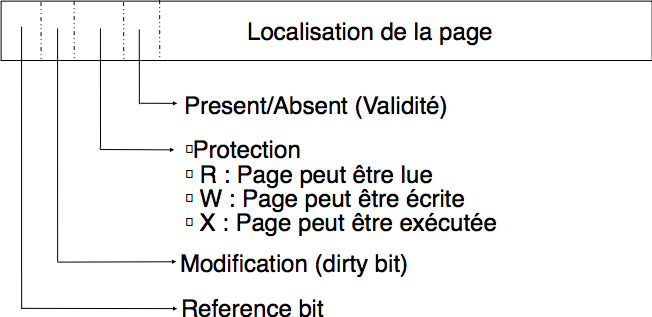
\includegraphics[width=\linewidth]{entreeComplete.png}
    \caption{Une entrée complète de la table des pages}
\end{figure}

Outre les bits de validité et de permission, une entrée de la table des
pages contient les bits de contrôle suivants :

\begin{itemize}
    \item le \textit{bit de référence} est mis à vrai par le
        \textit{MMU} dans le \textit{TLB} à chaque accès à une donnée se
        trouvant dans la page correspondante, que cet accès soit en
        lecture ou en écriture
    \item le \textit{bit de modification} ou \textit{dirty bit} est mis
        à vrai par le \textit{MMU} chaque fois qu'une opération
        d'écriture est réalisée dans cette page.
\end{itemize}

Ces deux bits sont mis à jour par le \textit{MMU} à l'intérieur du
\textit{TLB}. Lorsqu'une entrée de la table des pages est retirée du
\textit{TLB} pour être remise en mémoire, que ce soit à l'occasion d'un
changement de contexte ou parce que le \textit{TLB} est plein, les
valeurs de ces deux bits sont recopiées dans l'entrée correspondante
de la table des pages. En somme, le \textit{TLB} fonctionne comme une
cache en \textit{write-back} pour ces deux bits de contrôle.\newline
  
Les bits de référence et de modification sur utilisés par la plupart
des algorithmes de remplacement de pages. Le bit de référence est
généralement utilisé par le système d'exploitation pour déterminer
quelles sont les pages auxquelles un processus accède actuellement.
Pour cela, le noyau va régulièrement remettre à \textit{faux} les bits
de validité des entrées des tables de pages. Lorsque une entrée de la
table des pages est chargée dans le \textit{TLB} suite à un
\textit{page fault} son \textit{bit de référence} est mis à
\textit{vrai}. Il en va de même chaque fois que le processeur accède à
une donnée dans cette page. \newline
  
La stratégie de remplacement utilisant une \textit{file FIFO} que
nous avons mentionné précédemment peut être améliorée en utilisant le
\textit{bit de référence}. Plutôt que de remettre sur disque la page
dont l'identifiant est en tête de la file il suffit de regarder son
\textit{bit de référence}. Si celui-ci a la valeur \textit{faux}, la page n'a pas été utilisée récemment et peut
donc être retirée de la mémoire RAM. Sinon, le \textit{bit de référence}
est remis à \textit{faux} et l'identifiant de la page est
replacé en fin de file. L'algorithme de remplacement de page passe
ensuite à la page suivante dans la file et continue jusqu'à trouver
suffisamment de pages ayant leur bit de référence mis à
\textit{faux}.\newline
  
Une autre stratégie est de combiner le \textit{bit de référence} et
le \textit{dirty bit}. Dans ce cas, le noyau du système d'exploitation
va régulièrement remettre à la valeur\textit{faux} tous les bits de
référence (par exemple toutes les secondes). Lorsque la mémoire RAM est
pleine et qu'il faut libérer de l'espace mémoire pour charger de
nouvelles pages, l'algorithme de remplacement de pages va grouper les
pages en mémoire en quatre classes. \newline

\begin{enumerate}
    \item La première classe comprend les pages dont le \textit{bit de
        référence} et le \textit{bit de modification} ont comme valeur
        \textit{faux}. Ces pages n'ont pas été utilisées récemment et
        sont identiques à la version qui est déjà stockée sur disque.
        Elles peuvent donc être retirée de la mémoire RAM sans
        nécessiter de transfert vers le disque/
    \item La deuxième classe comprend les pages dont le \textit{bit de
        référence} a comme valeur \textit{faux} mais le \textit{bit de
        modification} a comme valeur \textit{vrai}. Ces pages n'ont pas
        été utilisées récemment, mais doivent être transférées vers le
        disque avant d'être retirées de la mémoire RAM.
    \item La troisième classe comprend les pages dont le \textit{bit de
        référence} a comme valeur \textit{vrai} mais le \textit{bit de
        modification} a comme valeur \textit{faux}. Ces pages ont été
        utilisées récemment mais peuvent être retirées de la mémoire RAM
        sans nécessiter de transfert vers le disque.
    \item La dernière classe comprend les pages dont les bits de
        référence et de modification ont comme valeur \textit{vrai}. Ces
        pages ont étés utilisées récemment et il faut les transférer
        vers le disque avant de les retirer de la mémoire RAM.
\end{enumerate}

Si l'algorithme de remplacement de pages doit retirer des pages de la
mémoire RAM, il commencera par retirer des pages de la première
classe, et ensuite de la deuxième, \ldots
  
Des algorithmes plus performants ont été proposés et sont utilisés en
pratique. Une description détaillée de ces algorithmes sort du cadre
de ce cours d'introduction mais peut être trouvée dans un livre
consacré aux systèmes d'exploitation comme \textit{Tannenbaum A,
Operating systems : design and implementation}.
  
\begin{framed}
  \textbf{Note} : Swapping et pagination \newline

  Grâce à l'utilisation de la mémoire virtuelle qui est découpée en
  pages, il est possible de stocker certaines parties de processus sur
  un dispositif de stockage plutôt qu'en mémoire RAM. Cette technique
  de \textbf{pagination} permet au système d'exploitation de gérer
  efficacement la mémoire et de réserver la mémoire RAM aux parties de
  processus qui sont nécessaires à leur exécution. Grâce à la découpe
  en pages, il est possible de transférer de petites parties d'un
  processus temporairement sur un dispositif de stockage. Aujourd'hui,
  la \textbf{pagination} est très largement utilisée, mais ce n'est pas
  la seule technique qui permette de placer temporairement l'espace
  mémoire utilisé par un processus sur disque. Le \textbf{swapping} est
  une technique plus ancienne mais qui est encore utilisée en pratique.
  Le \textbf{sapping} est plus radical que la \textbf{pagination}
  puisque cette technique permet au noyau de sauvegarder sur disque la
  quasi totalité de la mémoire utilisée par un processus. Le noyau fera
  appel au swapping lorsque la mémoire RAM est surchargée et pour des
  processus qui sont depuis longtemps bloqués par exemple en attente
  d'un opération d'entrée/sortie. Lorsque le noyau manque de mémoire, il
  est plus efficace de sauvegarder un processus complet plutôt que de
  transférer des pages de différents processus. Un tel processus swappé
  sera réactivé et ramené en mémoire par le noyau lorsqu'il repassera
  dans l'état \textit{Running}, par exemple suite à la réussite d'une
  opération d'entrée/sortie.
\end{framed}

\subsection{Qu'est-ce que la mémoire virtuelle ?}

In the good old days, the CPU directly accesses the physical memory

\begin{verb}
    loadbyte r0, 0x1001
\end{verb}

Address 0x1001 = byte \# 0x1001 of physical memory = physical address

\bigskip
\begin{tabular}{|l|l|l|l|l|l|}
    0 & 1 & \ldots & & & n - 1 \\
    \hline
    \ldots & \ldots & \ldots & & & \ldots \\
    \hline
\end{tabular}
\bigskip


\bigskip
\begin{itemize}
    \item Virtual memory
        \begin{itemize}
            \item Address 0x1001 is only a \textit{virtual address}
            \item Is translated into a physical address by a \textit{memory
                management unit} (MMU) : procédé magique qui traduit la
                VA 0x1001 -> MMU -> PA qu'on peut retrouver en mémoire.
        \end{itemize}
\end{itemize}
\bigskip

\subsubsection{Address Translation}

\begin{figure}[!ht]
    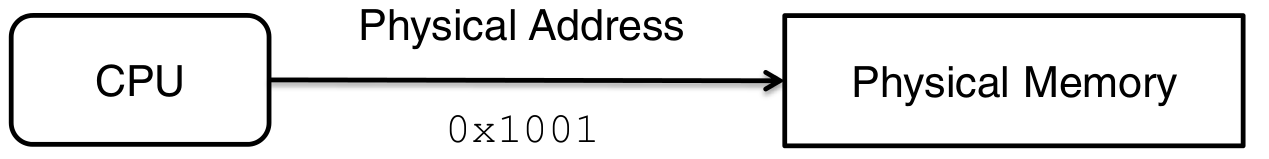
\includegraphics[width=\linewidth]{without_virtual_memory.png}
    \caption{Sans la mémoire virtuelle}
\end{figure}

\begin{figure}[!ht]
    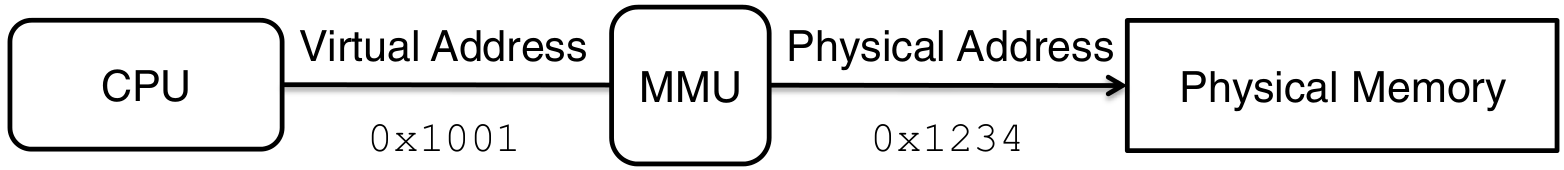
\includegraphics[width=\linewidth]{with_virtual_memory.png}
    \caption{Avec la mémoire virtuelle}
\end{figure}

Le CPU -> MMU -> MEMORY. Cette situation est tellement présente que
maintenant le MMU est intégré au CPU (depuis environ 20 ans).

\subsection{Why virtual memory ?}

\begin{itemize}
    \item Things you can do with virtual memory : on se sépare de la
        partie physique pour pouvoir travailler dans un programme avec
        des adresses virtuelles
        \begin{itemize}
            \item Per-process address spaces
            \item Shared memory: l'utilisation en est facilitée
            \item Memory protection
            \item Swapping
        \end{itemize}
\end{itemize}
\bigskip

\bigskip
\begin{itemize}
    \item Where is virtual memory NOT used ?
        \begin{itemize}
            \item First computers (quand on veut accéder à l'adresse, on
                tombe sur l'adresse réelle car ils n'ont pas de MMU).
            \item Simple systems (microcontrollers etc.)
        \end{itemize}
\end{itemize}
\bigskip

\subsection{Paged vs Segmented memory}

Historiquement, il existe deux approches à la mémoire virtuelle :

\begin{enumerate}
    \item La segmented memory (dépassé)
    \item La paged memory
\end{enumerate}

Segmented memory: ça existe pour des raisons historiques, c'est une
manière très particulière de faire de la virtualisation de mémoire. En
1970,les premiers CPU (Intel) avaient des pointeurs d'adresses en
16bit, ce qui fait qu'on ne peut accéder qu'à 64Kb ($2^{16}$) de mémoire physique.
\newline

Comment étendre le nombre d'adresses sans changer les hardwares ? Intel
a introduit le CPU 8086 en 1978, on utilise toujours des pointeurs
16bits, mais on peut avoir des adresses physiques de 20bits (le contenu
d'un registre de segment (\enquote{segment register}) est ajouté au
pointeur 16bit). On l'ajoute devant, ce qui permet de ne rien modifier
aux programmes qui existaient avant. Cette technique permet d'avoir
$2^{20}$ bytes (1MByte) d'adresses physiques.\newline

\begin{framed}
    \paragraph{Exemple} DS (data segment register, 16-bit) = 0x2000

    \verb#loadbyte r0, 0x1001#
    
    Adresse physique :

    \verb#0x2000<<4 + 0x1001 = 0x2000 + 0x1001 = 0x21001#
\end{framed}

Cette technique est très lourde : Data structures larger than 64Kb very hard to
implement. En effet, on doit modifier le registre qui permet
d'implémenter cette nouvelle méthode avant d'accéder à des adresses
mémoires. La seule raison pour laquelle ça existe, c'est parce que ça
permet la compatibilité (il suffit de mettre le DS à 0x0000). \newline

Intel a introduit un nouveau CPU en 1982. Il contient toujours des
registres de segment mais : \newline

\subsubsection{Les descriptor tables}

\paragraph{Intel 80286 CPU} sont introduits en 1982. Ils contiennent
toujours les registres de segment (segment registers), mais : 

\bigskip
\begin{itemize}
    \item 16-bit segment register interpreted as an index of interpreted
        as an index in a descriptor table
\end{itemize}
\bigskip

On va donc créer une table de déscripteurs (descriptor table) qui
contient des pointeurs vers la mémoire, ça permet de dire vers quelle
valeur les pointeurs dans les registres pointent dans la mémoire
physique. 24bit pointer in the Descriptor Table, 16 bits physical
address (segment). On y ajoute des flags pour dire si c'est du code à
exécuter, des données ou si la mémoire n'est pas utilisée. \newline

Une entrée dans la table des descripteurs (descriptor table) contient :

\begin{itemize}
    \item 24-bit physical base address of segment $\Rightarrow$ 24-bit
        address space (16 Mbytes)
    \item Size of segmenet (16 bit)
    \item Flags : executale (for code), writeable (for data), present
        (i.e. used \& not swapped to disk)
\end{itemize}

\begin{figure}[!ht]
    \centering
    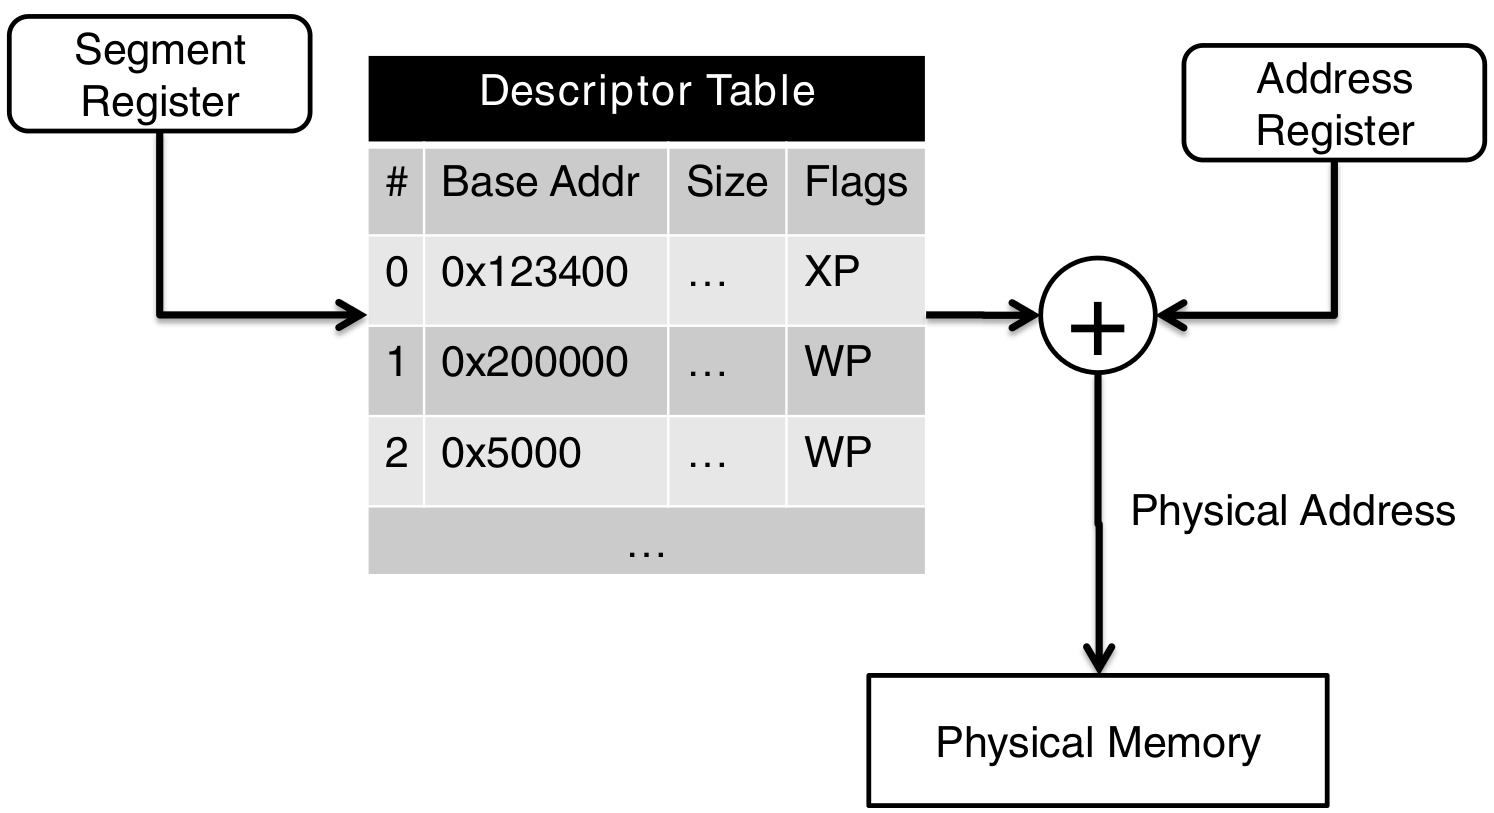
\includegraphics[width=\linewidth]{descriptor_table.png}
    \caption{Segmented memory : descriptor table}
\end{figure}

\begin{framed}
    \textbf{Exemple}

    \begin{itemize}
        \item DS (data segment register) = 0x0003
            \subitem \verb#loadbyte r0, 0x1001#
        \item Entry 3 in descriptor table :
            \begin{itemize}
                \item Base address = 0x123456
                \item Segment size = 0x2345
            \end{itemize}
        \item CPU checks size and flags of segment
        \item Physical address : 0x123456 + 0x1001 = 0x124457
    \end{itemize}
\end{framed}

Ce système a été étendu au système de pointeurs 32-bit et au paging. Le CPU a deux types de table : \newline

\bigskip
\begin{description}
    \item[Local table (LDT)] : one table per process, switched during
        process scheduling. Ca permet d'éviter des conflits d'accès
        mémoire car les descriptor table ne permettront pas de pointer
        vers des zones mémoires qui ne sont pas attribuées au processus.
        Le système d'exploitation (les vieux windows) ne permettent pas
        aux programmes d'utiliser les instructions lldt, lgdt ; c'est
        réservé au système d'exploitation uniquement, ça permet d'éviter
        qu'un programme accède aux données d'un autre programme (ce sont
        des niveaux de privilèges).
    \item[Global table (GDT)] : table for the entire system
\end{description}
\bigskip

Il existe des instructions spéciales permettant de charger les tables :

\begin{framed}
\verb#lldt <address of table>#

\verb#lgdt <address of table>#
\end{framed}

Les local LDTs créent des espaces d'adressage séparés et une protection
mémoire pour les processus :

\begin{figure}[!ht]
    \centering
    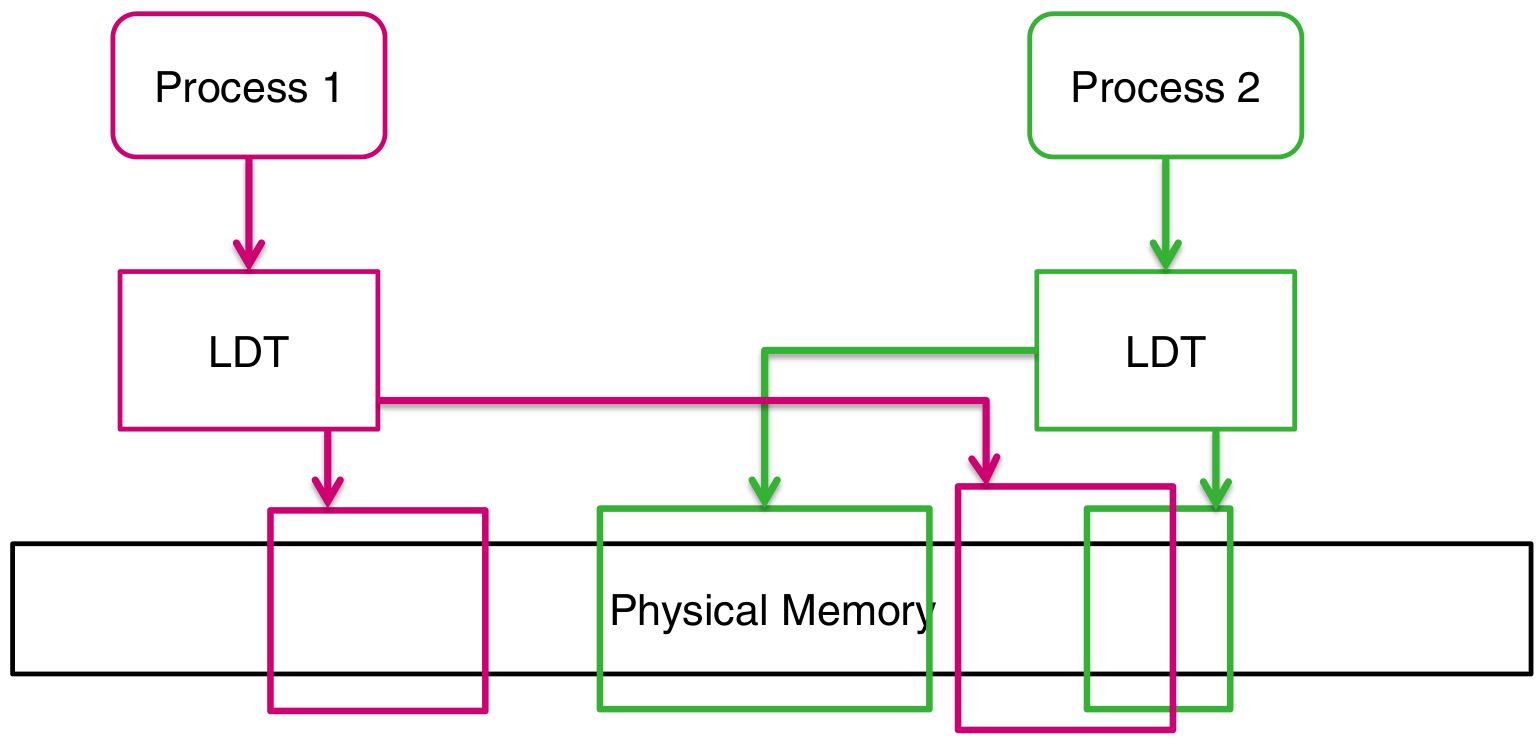
\includegraphics[width=\linewidth]{multiple_local_descriptor_tables.png}
    \caption{Multiple local descriptor tables for processes}
\end{figure}

\subsection{Les niveaux de privilèges}

Les CPU Intel ont 4 niveaux de privilèges :

\bigskip
\begin{itemize}
    \item Ring 0 : OS kernel code (seul à posséder certaines
        instructions comme \verb#lgdt#, privileged instruction)
    \item Ring 1,2 : not used anymore, originally for drivers, etc.
    \item Ring 3 : User code
\end{itemize}
\bigskip

Les autres CPU ont des concepts similaires, typiquement :

\bigskip
\begin{itemize}
    \item User mode : for user applications
    \item Privileged/Supervisor mode : for OS kernel
\end{itemize}
\bigskip

Les segment descriptors contiennent des informations des ring. Un ring
ne peut pas accéder à des données du ring inférieur. \newline

\subsection{Résumé}

Les adresses virtuelles sont traduites en adresses physiques à travers
les descriptor tables. Les LDT permettent d'avoir des espaces d'adresses
séparés pour chaque processus et donc la protection de leur mémoire (on
évite que les processus puissent écrire sur la mémoire d'autres
processus). La GDT est utilisé uniquement par l'OS ou par la shared
memory. La mémoire segmentée est flexible : elle peut avoir une taille
de segment variable. Les segments peuvent être swappés sur un disque
dur, mais le coût de ce swapping est difficile à prévoir à cause de la
taille de segment variable.

\subsection{La mémoire segmentée aujourd'hui}

La segmented memory n'est plus utilisée aujourd'hui. Maintenant, on
utilise le Paging (mais le segmented existe toujours). \newline

\begin{framed}
    \paragraph{Exemple} From the GRUB boot loader :

    \begin{verbatim}
gdt_entry_t gdt_entries[5];
...
gdt_set_gate(0,0,0,0,0);                // Null segment
gdt_set_gate(1,0,0xFFFFFFFF,0x9A,0xCF); // Code segment
gdt_set_gate(2,0,0xFFFFFFFF,0x92,0xCF); // Data segment
gdt_set_gate(3,0,0xFFFFFFFF,0xFA,0xCF); // User code segment
gdt_set_gate(4,0,0xFFFFFFFF,0xF2,0xCF); // User data segment
gtd_ptr.limit = 5*8-1               // 5 entries of 8 bytes
gdt_ptr.base = &gdt_entry;          // the GDT
lgdt gdt_ptr                        // (assembly instruction)
    \end{verbatim}
\end{framed}

Les instructions créent un segment pour le code, les données, les
processus. Les segments existent donc toujours mais en fait ils ne sont
plus utiles (c'est juste pour que le processeur ne plante pas). \newline

